

%MOST BASIC DOCUMENT
\documentclass[14pt, a4paper]{article} %14 pt indicates the font size of the prepared document
\usepackage[utf8]{inputenc} %indicates the encoding of the document
\begin{document}
	This is the first document.
\end{document}



%TITLE, AUTHOR, DATE
% \documentclass[14pt, a4paper]{article} %14 pt indicates the font size of the prepared document
% \usepackage[utf8]{inputenc} %indicates the encoding of the document
% \title{Introductory Class on Latex}
% \author{Mahjabin Nahar}
% \date{\today}
% \date{21 March 2021}

% \begin{document}
% \maketitle
% \end{document}



%SECTION, SUBSECTION, PARAGRAPH, TABLE OF CONTENTS, AND SOME FORMATTING EXAMPLES
% \documentclass[14pt, a4paper]{article} %14 pt indicates the font size of the prepared document
% \usepackage[utf8]{inputenc} %indicates the encoding of the document
% \usepackage{color} %this package enables the use of colors.

% \title{Introductory Class on Latex}
% \author{Mahjabin Nahar}
% \date{\today}
% \date{21 March 2021}

% \begin{document}
% \maketitle
% \tableofcontents %this command creates the table of contents with all numbered sections, subsections, etc.
% \pagebreak %This will force the rest of the document to start in another page.

% \section{Introduction}
% This is the introduction section.

% \subsection{Subsection 1.1}
% This is subsection 1.1.

% This sentence will begin in a new paragraph due to the blank line before it. This is a filler line.\par
% However, this sentence begins in a new paragraph due to the \\par command used after the end of the last sentence. This is another filler line.

% \subsubsection{Subsubsection 1.1.1}
% This is subsubsection 1.1.1.

% \subsection*{Unnumbered subsection}
% This is an unnumbered subsection under Introduction. \textbf{This will NOT show up in the Table of Contents.} 

% \emph{This sentence is an example of emphasis. Even though it is italic in this example, using another package might change it to something else, like underlined text.  \emph{Also, emphasis can be nested.} The previous sentence was an example of nested emphasis.} 

% \textit{This sentence will always be italic.}
% %\color{red} This is a red sentence. %This command will make the rest of document red (including this sentence) 
% {\color{red} This is a red sentence.} %This command will only make this sentence red


% \section*{Unnumbered Section Example}
% This section should not be numbered. Using * after the section specifier prevents this numbering. This will NOT show up in the Table of Contents.
% \LARGE{This sentence is LARGE.}
% \Huge{This sentence is HUGE.}

% \end{document}



% DIFFERENT TYPES OF LISTS, FIGURES, AND REFERENCING (SECTIONS, FIGURES, ETC.)
% \documentclass[14pt, a4paper]{article} %14 pt indicates the font size of the prepared document
% \usepackage[utf8]{inputenc} %indicates the encoding of the document
% \usepackage{color} %this package enables the use of colors.
% \usepackage{graphicx}

% \title{Introductory Class on Latex}
% \author{Mahjabin Nahar}
% \date{\today}
% \date{21 March 2021}

% \begin{document}
% \maketitle
% \tableofcontents %this command creates the table of contents with all numbered sections, subsections, etc.
% \pagebreak %This will force the rest of the document to start in another page.

% \section{Section 1}
% \label{sec:intro} %This will be used while referencing this section
% This is the introduction section.

% This is an itemized list.
% \begin{itemize}
%     \item item 1
%     \begin{itemize}
%         \item nested item 1
%         \item nested item 2
%     \end{itemize}
%     \item item 2
%     \item item 3
% \end{itemize}

% \subsection{Subsection 1.1}
% \label{subsec:1.1} %This will be used while referencing this subsection
% This is subsection 1.1.

% This is an enumerated list.
% \begin{enumerate}
%     \item First item
%     \item Second item
%     \item This can also be nested.
%     \begin{enumerate}
%         \item nested item 1
%         \item nested item 2
%     \end{enumerate}
% \end{enumerate}

% \subsubsection{Subsubsection 1.1.1}
% This is subsubsection 1.1.1.

% This is a descriptive list.
% \begin{description}
% \item[Number 1] one
% \item[Number 2] two
% \end{description}

% \pagebreak 

% \subsection*{Unnumbered subsection}
% This is an unnumbered subsection under Introduction. 
% \begin{figure}[h]
% 	\centering
% 	\caption{This caption is at the top}
% 	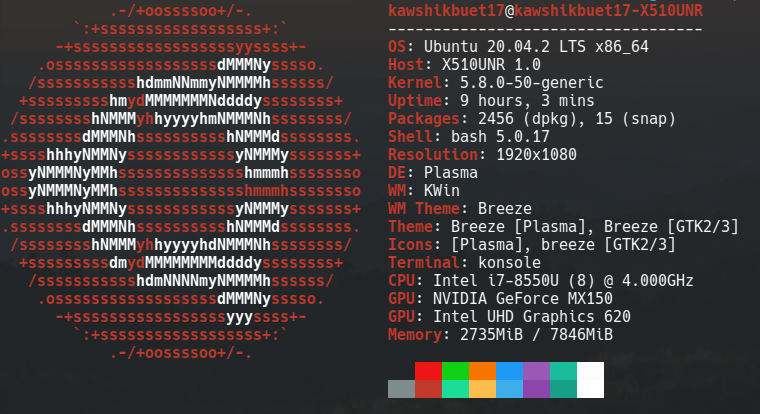
\includegraphics[scale=0.4]{figure1.jpg}
% 	\label{fig:1}
% 	%\caption{This is figure 1.}
% \end{figure}


% \section*{Unnumbered Section Example}
% This section should not be numbered. Using * after the section specifier prevents this numbering. This will NOT show up in the Table of Contents. 

% Referencing the figure used above: \ref{fig:1}.

% \end{document}


%TABLES, MULTIROW, MULTICOLUMN   
% \documentclass[14pt, a4paper]{article} %14 pt indicates the font size of the prepared document
% \usepackage[utf8]{inputenc} %indicates the encoding of the document
% \usepackage{multicol}
% \usepackage{multirow}

% \title{Introductory Class on Latex}
% \author{Mahjabin Nahar}
% \date{\today}
% \date{21 March 2021}

% \begin{document}
% \maketitle
% \tableofcontents %this command creates the table of contents with all numbered sections, subsections, etc.
% \pagebreak %This will force the rest of the document to start in another page.

% \section{Section 1}
% \label{sec:intro} %This will be used while referencing this section
% This is the introduction section.


% \subsection{Subsection 1.1}
% \label{subsec:1.1} %This will be used while referencing this subsection
% This is subsection 1.1.


% \subsubsection{Subsubsection 1.1.1}
% This is subsubsection 1.1.1.


% \subsection*{Unnumbered subsection}
% This is an unnumbered subsection under Introduction. 

% \section{Table}

% \begin{tabular}{|c|c|c|c|}
%     \hline
% 	1 & 2 & 3 & 4 \\ 
% 	\cline{1-3}
% 	1 & 2 & 3 & 4  \\
% 	\hline
% 	\multicolumn{3}{|c|}{text} & 4 \\
% 	\hline
% 	\multirow{2}{*}{text} & 2 & 3 & 4\\
% 	\cline{2-4}
% 	& 2 & 3 & 4 \\
% 	\hline
% 	\multicolumn{3}{|c|}{\multirow{2}{*}{text}} & 5 \\
% 	\multicolumn{3}{|c|}{} & 7 \\
% 	\hline
% \end{tabular}

% \subsection{Basic Table}
% \begin{tabular}{|c|ccc|}
% 	\hline
% 	1 & 2 & 3 & 4 \\ 
% 	\cline{1-3}
% 	1 & 2 & 3 & 4  \\
% 	\hline

% \end{tabular}


% \subsection{Multi-column Table}

% \begin{tabular}{|c|ccc|}
% 	\hline
% 	1 & \multicolumn{3}{c|}{text} \\ 
% 	\cline{2-4}
% 	1 & 2 & 3 & 4  \\
% 	\hline

% \end{tabular}


% \subsection{Multi-row Table}

% \begin{tabular}{|c|c|c|}
% 	\hline
% 	1 & 2 & 3 \\ 
% 	\hline
% 	\multirow{2}{*}{text} & 4 & 5 \\
% 	& 6 & 7 \\ 
% 	\hline


% \end{tabular}

% \subsection{Both}

% \begin{tabular}{|cc|c|}
% 	\hline
% 	1 & 2 & 3 \\ 
% 	\hline
% 	\multicolumn{2}{|c|}{\multirow{2}{*}{text}} & 5 \\
% 	& & 7 \\
% 	\hline
% \end{tabular}

% \end{document}

%EQUATION and MATH MODE
% \documentclass[16pt, a4paper]{article} %14 pt indicates the font size of the prepared document
% \usepackage[utf8]{inputenc} %indicates the encoding of the document
% \usepackage{amsmath}

% \title{Introductory Class on Latex}
% \author{Mahjabin Nahar}
% \date{\today}
% \date{21 March 2021}

% \begin{document}
% \maketitle
% \tableofcontents %this command creates the table of contents with all numbered sections, subsections, etc.
% \pagebreak %This will force the rest of the document to start in another page.

% \section{Equation}
% This is a simple equation: $a + a = 2a$

% \section{Superscript and Subscript}
% Superscript: $a^n$, $a^{in}$
% \newline
% Subscript: $a_n$, $a_{in}$
% \newline
% Nested Superscript and Subscript: $a^{b^n}$, $a_{b_n}$

% \section{Mathematical Environments}
% Inline: $\sum_{i=0}^n a_i$
% \newline
% Inline with displaystyle: $\displaystyle\sum_{i=0}^n a_i$
% \newline
% Block level: $$\sum_{i=0}^n a_i$$
% \newline
% Block level with equation number:
% \begin{equation}
% \sum_{i=0}^n a_i
% \end{equation}

% \section{Miscellaneous}
% Comparisons:
% $ <$, $ \leq $, $ > $, $\geq $
% \newline
% Union and Intersection:
% $A \cap B$, $A \cup B$
% \newline
% Fractions: $\frac{a}{b}$, ($\frac{a}{b}$), $\left(\frac{a}{b}\right)$

% \end{document}


%Bibliography
% \documentclass[16pt, a4paper]{article} %14 pt indicates the font size of the prepared document
% \usepackage[utf8]{inputenc} %indicates the encoding of the document
% \usepackage{biblatex}
% \addbibresource{ref.bib}

% \title{Introductory Class on Latex}
% \author{Mahjabin Nahar}
% \date{\today}
% \date{21 March 2021}

% \begin{document}
% \maketitle
% \tableofcontents %this command creates the table of contents with all numbered sections, subsections, etc.
% \pagebreak %This will force the rest of the document to start in another page.

% \section{Bibliography}
% This section cites Einstein's journal paper \cite{einstein} and Dirac's book \cite{dirac}. 

% \printbibliography


% \end{document}